\subsection{Decision Tree Algorithm}

A binary decision tree is a hierarchical structure that takes input data at its root and propagates it to one of many leaves. Each \emph{leaf} of the tree represents a class designation. To reach a leaf, the features of the data are utilized at \emph{nodes} to make a binary decision: to proceed down the left or right \emph{branch} of the tree? To answer this question, the node also carries a \emph{threshold} that the feature value of the test data is compared against. If the test feature is less than the threshold, we proceed down the left branch. Otherwise, the right. An illustration of a simple decision tree is pictured below.
%
\begin{figure}[H]
  \centering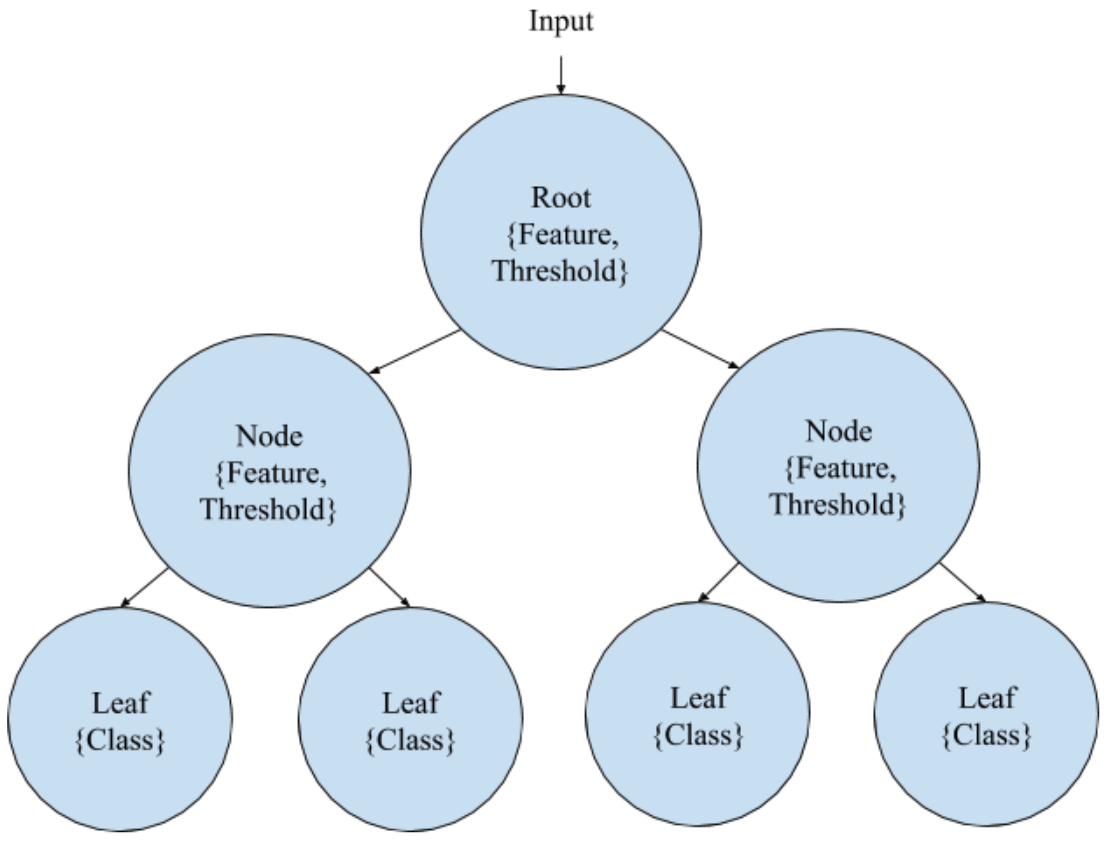
\includegraphics[width=0.6\columnwidth]{../images/decision_tree}
  \caption{An example decision tree.}
\end{figure}

This decision tree structure needs to be generated before it can be used with test data. To train a decision tree that appropriately classifies our test data according to the features we generated, we employ a recursive function. The function signature is
%
\begin{equation*}
  \mathtt{tree = trainDecisionTree(set)}
\end{equation*}

Where \code{set} is the training set, which is a MATLAB structure that contains the raw data (unused), class labels, and generated features. \code{tree} is the returned structure that can be used during testing. It is essentially a nested structure that contains two types of elements: nodes and leaves. At each node of the tree, a feature and threshold are specified. If a test sample's value at that particular feature is less than the threshold, the sample is passed down the left branch of the node. Similarly, if the sample's feature is greater than the threshold, it goes through the right branch. This is repeated until we reach a leaf node, which specifies a class membership. 

The decision tree training algorithm has a few major steps, and proceeds by evaluating a metric called \emph{information gain} at various configurations. For now, suffice it to say that information gain is a scalar that represents the improvement in prediction as we narrow down the set (by growing the tree) to find appropriate leaves. Our implementation most closely follows that of the ID3 and C4.5 algorithms developed by Ross Quinlan in the late 80s and early 90s \cite{wiki:id3} \cite{wiki:c45}.
%
\begin{enumerate}
\item Check stopping conditions, which generate leaves.
%
  \begin{itemize}
  \item If there are no more features to split on, return a leaf with the class mode of the set. 
  \item The set is smaller than \code{minLeaf}, which is a tuning parameter that is meant to reduce overfitting of the training data. If this condition is met, return a leaf with the class mode of the set.
  \item If all samples in the set belong to the same class, return a leaf with the class.
  \item If no feature yields an improvement to the information gain (discussed below), then return a leaf with the class mode of the set. Note that this condition is only evaluated after step 2. 
  \end{itemize}
\item Iterate over each feature. Sort the set along the current feature. We utilize a threshold that splits the set between adjacent feature values. Because the information gain across thresholds is convex on the whole (see Fig. \ref{fig:IG}), we use a line search that approximates the highest information gain for each threshold. 

  Let \code{attributeBest} and \code{indBest} be the feature and index that yield the highest information gain. Since the set is sorted, we can simply split the set at the index given by \code{indBest} for the recursion.
\item Recur over the subsets given by \code{indBest} to find the next attribute that yields the highest information gain. Note that we exclude the attribute/feature we chose in this execution of \code{trainDecisionTree(.)}. 
\end{enumerate}

The algorithm is reproduced in pseudocode below.

\begin{algorithm}[H]
\DontPrintSemicolon
\KwData{\textit{set} of training samples with class labels ($set(1)$) and attributes (features) ($set(2)$).\\
  \textit{minLeaf}, an integer specifying the minimum number of elements in \textit{set} required to make a splitting node. \textit{i.e.} a leaf is generated if the set has fewer elements than \textit{minLeaf}.
}
\KwResult{\textit{tree}, a structure containing nodes and leaves.}
\Begin{
  check for base cases:\;
  \If{$set(2) = \emptyset$}{
    no more attributes (features) to split on.\;
    {\bf return} \textit{leaf} with mode of $set(1)$ (class labels)\;
  }
  \If{$length(set(1)) < minLeaf$}{
    {\bf return} \textit{leaf} with mode of $set(1)$ (class labels)\;
  }
  
  $thisSetEntropy \longleftarrow getEntropy(set)$\;
  \If{{\bf not} thisSetEntropy}{
    all samples are in the same class.\;
    {\bf return} \textit{leaf} with first element of $set(1)$\;
  }
  \;
  instantiate tracking variables:\;
  $attributeBest \longleftarrow 0$\;
  $thresholdBest \longleftarrow 0$\;
  \textit{infoGainBest} $\longleftarrow 0$\;
  $indexBest \longleftarrow 0$\;

  \For{attribute $\in$ range(\# of features left in set)}{
    sort \textit{set} along $attribute$.\;
    perform line search heuristic to approximate max information gain by splitting $set$ at various indices.\;
    \textit{thisInfoGain} $\longleftarrow$ \textit{lineSearch(set)}
    \;
    \If{thisInfoGain $>$ infoGainBest}{
      $attributeBest \longleftarrow attribute$\;
      \textit{infoGainBest} $\longleftarrow$ \textit{thisInfoGain}\;
      $indexBest \longleftarrow$ index given by line search\;      
      $thresholdBest \longleftarrow$ attribute value midway between $indexBest$ and $indexBest + 1$\;
    }
  }
  \;
  \If{{\bf not} infoGainBest {\bf or} {\bf not} attributeBest}{
    no attribute provides an information gain.\;
    {\bf return} \textit{leaf} with mode of $set(1)$ (class labels)\;
  }
  \;
  re-sort $set$ along $attributeBest$.\;
  $subsets \longleftarrow getSubsets(set, attributeBest, indexBest)$\;
  $subtree1 \longleftarrow trainDecisionTree(subsets(1), minLeaf)$\;
  $subtree2 \longleftarrow trainDecisionTree(subsets(2), minLeaf)$\;
  \;
  {\bf return} \textit{node} with $attributeBest$, $thresholdBest$, $subtree1$, and $subtree2$\;
}
\caption{trainDecisionTree} \label{alg:dt}
\end{algorithm}

%\pagebreak
Once we have trained the decision tree, we can begin to test it by passing the features generated from the test set through the tree. The testing algorithm is reproduced in psuedocode below.

\begin{algorithm}[H]
\DontPrintSemicolon
\KwData{
  \textit{set} of test samples with class labels ($set(1)$) and attributes (features) ($set(2)$).\\
  \textit{tree}, the struct of structs that represents the trained decision tree.
}
\KwResult{\textit{set}, the input structure modified to include predicted class membership.}
\Begin{
  \For{{\bf each} $sample \in set$}{
    \textit{treeWalked} $\longleftarrow$ \textit{tree}\;
    \textit{classified} $\longleftarrow$ false\;
    \textit{attributes} $\longleftarrow$ features corresponding to this sample\;
    \
    \While{{\bf not} classified}{
     \If{treeWalked {\bf is a} node}{
       \textit{thisAttribute} $\longleftarrow$ attribute given by \textit{treeWalked}\;
       \textit{thisAttributeValue} $\longleftarrow$ value of the sample's feature at \textit{thisAttribute}\;
       \textit{thisThreshold} $\longleftarrow$ threshold given by \textit{treeWalked}\;
       \
       {\bf remove} \textit{thisAttribute} from the sample's feature vector.\;
       {\bf compare} \textit{thisAttributeValue} to \textit{thisThreshold}:\;
       \If{thisAttributeValue $<$ thisThreshold}{
         choose left branch.\;
         \textit{treeWalked} $\longleftarrow$ left branch given by current \textit{treeWalked}.\;
       }
       \Else{
         choose right branch.\;
         \textit{treeWalked} $\longleftarrow$ right branch given by current \textit{treeWalked}.\;
       }
     }
     \Else{
       \textit{treeWalked} is a leaf.\;
       append predicted label to $set(2)$ at this sample.\;
       \textit{classified} $\longleftarrow$ true\;
     }
    }
  }
}
\caption{testDecisionTree} \label{alg:dt_test}
\end{algorithm}

\subsubsection{Entropy and Information Gain}

When growing the decision tree, the training algorithm utilizes a metric called \emph{information gain} to optimize the predictive power of the tree. Before we can define information gain, we must first understand \emph{entropy.} Entropy is an information theoretic concept that represents the amount of uncertainty in a given set of data. It is defined as
%
\begin{equation}
  \mathrm{H}(X) = -\sum_{i=1}^n {\mathrm{P}(x_i) \log_2 \mathrm{P}(x_i)}
\end{equation} 

Where $\mathrm{P}(x_i)$ is the proportion of the number of elements with class $x_i$ to the number of elements in the set $X$. there are $n$ classes in the set. Note that if all samples belong to class $i$, $\mathrm{P}(x_i) = 1$ and $\log_2 \mathrm{P}(x_i) = 0$, so the entropy is zero. 

In calculating the information gain of splitting the set into two subsets, we utilize the entropy of the parent set and subtract from it a weighted entropy of each subset. This is better expressed by the following equation:
%
\begin{equation}
  \mathrm{IG}(X) = \mathrm{H}(X) - \sum_{i=1}^{2} \frac{|S_i|}{|X|} \mathrm{H}(S_i)
\end{equation}

Where $|\cdot|$ is the cardinality, or number of elements in the set, and $S_i$ are the two subsets composed of the elements of $X$ partitioned across a given threshold for a given feature. The figure below is a plot of the information gain across splitting indices. So, after partitioning the set across a single attribute, (all elements of $S_1$ are less than the threshold, and all elements in $S_2$ are greater), we have a scalar value of information gain to decide which splitting threshold and feature would most improve the predictive ability of the decision tree. The plot below represents just one feature, but this calculation is required across all currently available features in the set. This quickly becomes computationally taxing for a large data-set, so we utilize a line search heuristic to improve the computational time without sacrificing a significant amount of accuracy. 

The line search starts in the middle of the set and splits it, computing an information gain (IG). Then, we compare this middle IG to the IGs obtained by splitting the set at the 25\% and 75\% indices. If either of these reveals a larger IG, we set it to the new 'middle' index and consider the IGs which emerge from splitting the set half-way between the old 'middle' and half-way between the old 'left' or 'right' (depending on which one yielded a larger IG.) This allows us to approximate the maximum value of the information gain for a given feature without a brute-force technique of considering each threshold. We ensured that the line search incorporates a variety of locations to coax it to approaching the global maximum, rather than getting caught in the minor variations between adjacent indices.  
%
\begin{figure}[H]
  \centering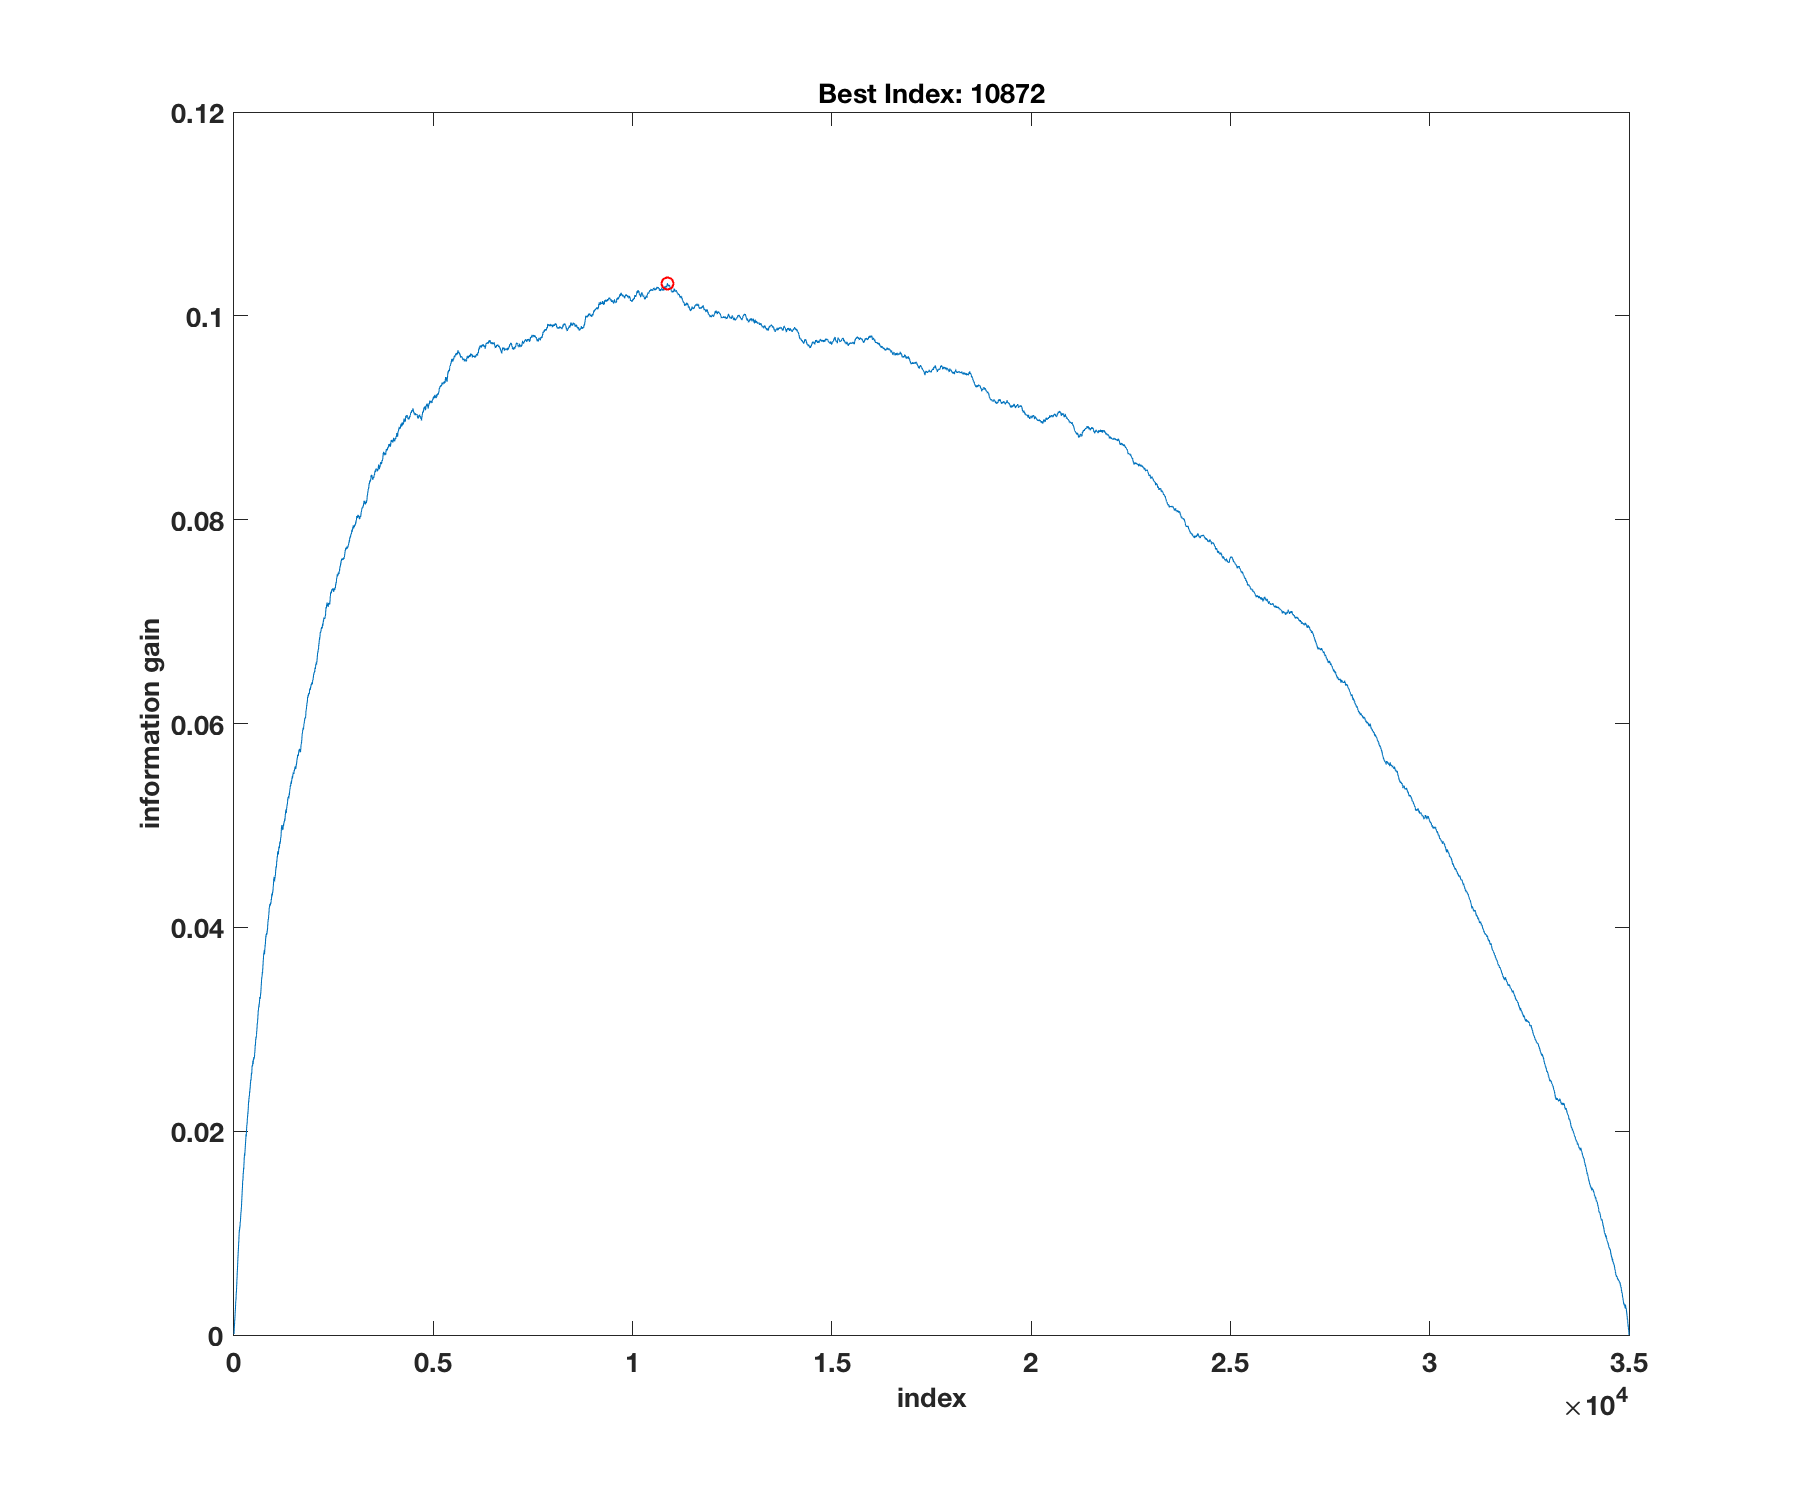
\includegraphics[width=0.6\columnwidth]{../images/IG}
  \caption{Information Gain across all possible thresholds.}
  \label{fig:IG}
\end{figure}
